% Chapter 7: Cointegration and VECM
% Harvard-quality academic presentation
% Bachelor program, Bucharest University of Economic Studies

\documentclass[9pt, aspectratio=169, t]{beamer}

% Ensure content fits on slides
\setbeamersize{text margin left=8mm, text margin right=8mm}

%=============================================================================
% THEME AND STYLE CONFIGURATION
%=============================================================================
\usetheme{default}
% Using default theme for clean header/footer control

% Color Palette (matching Redispatch PDF)
\definecolor{MainBlue}{RGB}{26, 58, 110}
\definecolor{AccentBlue}{RGB}{26, 58, 110}
\definecolor{IDAred}{RGB}{205, 0, 0}
\definecolor{DarkGray}{RGB}{51, 51, 51}
\definecolor{MediumGray}{RGB}{128, 128, 128}
\definecolor{LightGray}{RGB}{248, 248, 248}
\definecolor{VeryLightGray}{RGB}{235, 235, 235}
\definecolor{KeynoteGray}{RGB}{218, 218, 218}
\definecolor{SectionGray}{RGB}{120, 120, 120}
\definecolor{FooterGray}{RGB}{100, 100, 100}
\definecolor{Crimson}{RGB}{220, 53, 69}
\definecolor{Forest}{RGB}{46, 125, 50}
\definecolor{Amber}{RGB}{181, 133, 63}
\definecolor{Orange}{RGB}{230, 126, 34}
\definecolor{Purple}{RGB}{142, 68, 173}

% Gradient background (exact Keynote 315° gradient: white to RGB 218,218,218)
\setbeamertemplate{background}{%
    \begin{tikzpicture}[remember picture, overlay]
        \shade[shading=axis, shading angle=315,
        top color=white, bottom color=KeynoteGray]
        (current page.south west) rectangle (current page.north east);
    \end{tikzpicture}%
}
% Fallback solid color for compatibility
\setbeamercolor{background canvas}{bg=}

\setbeamercolor{palette primary}{bg=MainBlue, fg=white}
\setbeamercolor{palette secondary}{bg=MainBlue!85, fg=white}
\setbeamercolor{palette tertiary}{bg=MainBlue!70, fg=white}
\setbeamercolor{structure}{fg=MainBlue}
\setbeamercolor{title}{fg=IDAred}
\setbeamercolor{frametitle}{fg=IDAred, bg=}
\setbeamercolor{block title}{bg=MainBlue, fg=white}
\setbeamercolor{block body}{bg=VeryLightGray, fg=DarkGray}
\setbeamercolor{block title alerted}{bg=Crimson, fg=white}
\setbeamercolor{block body alerted}{bg=Crimson!8, fg=DarkGray}
\setbeamercolor{block title example}{bg=Forest, fg=white}
\setbeamercolor{block body example}{bg=Forest!8, fg=DarkGray}
\setbeamercolor{item}{fg=MainBlue}

% Footer colors (override Madrid theme blue)
\setbeamercolor{author in head/foot}{fg=FooterGray, bg=}
\setbeamercolor{title in head/foot}{fg=FooterGray, bg=}
\setbeamercolor{date in head/foot}{fg=FooterGray, bg=}
\setbeamercolor{section in head/foot}{fg=FooterGray, bg=}
\setbeamercolor{subsection in head/foot}{fg=FooterGray, bg=}

% Bullet styles (apply everywhere including blocks)
\setbeamertemplate{itemize item}{\color{MainBlue}$\boxdot$}
\setbeamertemplate{itemize subitem}{\color{MainBlue}$\blacktriangleright$}
\setbeamertemplate{itemize subsubitem}{\color{MainBlue}\tiny$\bullet$}
\setbeamertemplate{itemize/enumerate body begin}{\normalsize}
\setbeamertemplate{itemize/enumerate subbody begin}{\normalsize}

% Item spacing - compact style
\setlength{\leftmargini}{10pt}       % Level 1: minimal indent
\setlength{\leftmarginii}{10pt}      % Level 2: minimal additional indent
% Compact list spacing (zero extra space before/after lists in blocks)
\makeatletter
\def\@listi{\leftmargin\leftmargini \topsep 0pt \parsep 0pt \itemsep 0pt}
\def\@listii{\leftmargin\leftmarginii \topsep 0pt \parsep 0pt \itemsep 0pt}
\makeatother

\setbeamertemplate{navigation symbols}{}

%=============================================================================
% CUSTOM HEADLINE
%=============================================================================
\setbeamertemplate{headline}{%
    \vskip10pt%
    \hbox to \paperwidth{%
        \hskip0.5cm%
        {\small\color{FooterGray}\renewcommand{\hyperlink}[2]{##2}\insertsectionhead}%
        \hfill%
        \textcolor{FooterGray}{\small\insertframenumber}%
        \hskip0.5cm%
    }%
    \vskip4pt%
    {\color{FooterGray}\hrule height 0.4pt}%
}

%=============================================================================
% CUSTOM FOOTER
%=============================================================================
\usepackage{fontawesome5}

\setbeamertemplate{footline}{%
    {\color{FooterGray}\hrule height 0.4pt}%
    \vskip4pt%
    \hbox to \paperwidth{%
        \hskip0.5cm%
        \textcolor{FooterGray}{\small Time Series Analysis and Forecasting}%
        \hfill%
        \raisebox{-0.1em}{%
            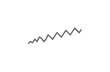
\begin{tikzpicture}[x=0.08em, y=0.08em, line width=0.4pt]
                \draw[FooterGray] (0,3) -- (1,4) -- (2,3.5) -- (3,5) -- (4,4) -- (5,6) -- (6,5.5) -- (7,4) -- (8,5) -- (9,7) -- (10,6) -- (11,5) -- (12,6.5) -- (13,8) -- (14,7) -- (15,6) -- (16,7.5) -- (17,9) -- (18,8) -- (19,7) -- (20,8.5) -- (21,10) -- (22,9) -- (23,8) -- (24,9.5);
            \end{tikzpicture}%
        }%
        \hskip0.5cm%
    }%
    \vskip6pt%
}

%=============================================================================
% PACKAGES
%=============================================================================
\usepackage[utf8]{inputenc}
\usepackage[T1]{fontenc}
\usepackage{amsmath, amssymb, amsthm}
\usepackage{mathtools}
\usepackage{bm}
\usepackage{tikz}
\usetikzlibrary{arrows.meta, positioning, shapes, calc, decorations.pathreplacing, shadings}
\usepackage{booktabs}
\usepackage{multirow}
\usepackage{array}
\usepackage{graphicx}
\usepackage{hyperref}
\usepackage{colortbl}
\hypersetup{colorlinks=true, linkcolor=MainBlue, urlcolor=MainBlue}
\graphicspath{{../../logos/}{../../charts/}}
\hfuzz=2pt  % Suppress tiny overfull warnings (<2pt)
\vfuzz=2pt  % Suppress tiny vertical overfull warnings (<2pt)

%=============================================================================
% QUANTLET COMMAND
%=============================================================================
\newcommand{\quantlet}[2]{%
    \hfill\href{#2}{%
        \raisebox{-0.15em}{\includegraphics[height=0.7em]{ql_logo.png}}%
        \textcolor{MainBlue}{\tiny\ #1}%
    }%
}

%=============================================================================
% CUSTOM TITLE PAGE
%=============================================================================
\defbeamertemplate*{title page}{hybrid}[1][]
{
    \vspace{0.2cm}
    % Logos row - top header (with clickable links)
    \begin{center}
        \href{https://www.ase.ro}{\includegraphics[height=1.0cm]{ase_logo.png}}\hspace{0.3cm}%
        \href{https://theida.net}{\includegraphics[height=1.0cm]{ida_logo.png}}\hspace{0.3cm}%
        \href{https://blockchain-research-center.com}{\includegraphics[height=1.0cm]{brc_logo.png}}\hspace{0.3cm}%
        \href{https://www.ai4efin.ase.ro}{\includegraphics[height=1.0cm]{ai4efin_logo.png}}\hspace{0.3cm}%
        \href{https://ipe.ro/new}{\includegraphics[height=1.0cm]{acad_logo.png}}\hspace{0.3cm}%
        \href{https://www.digital-finance-msca.com}{\includegraphics[height=1.0cm]{msca_logo.png}}%
    \end{center}

    \vspace{0.6cm}

    % Main title with Q logos on sides (with clickable links)
    \begin{center}
        \begin{minipage}{0.1\textwidth}
            \centering
            \href{https://quantlet.com}{\includegraphics[height=1.1cm]{ql_logo.png}}
        \end{minipage}%
        \begin{minipage}{0.78\textwidth}
            \centering
            {\LARGE\bfseries\usebeamercolor[fg]{title}\inserttitle}

            \vspace{0.3cm}

            {\usebeamerfont{subtitle}\usebeamercolor[fg]{title}\insertsubtitle}
        \end{minipage}%
        \begin{minipage}{0.1\textwidth}
            \centering
            \href{https://quantinar.com}{\includegraphics[height=1.1cm]{qr_logo.png}}
        \end{minipage}
    \end{center}

    \vspace{0.6cm}

    % Authors (left aligned)
    \hspace{0.5cm}{\usebeamerfont{author}\insertauthor}

    \vspace{0.3cm}

    % Institute/Affiliations (left aligned)
    \hspace{0.5cm}\begin{minipage}[t]{0.9\textwidth}
        \raggedright\small\insertinstitute
    \end{minipage}
}

%=============================================================================
% THEOREM ENVIRONMENTS
%=============================================================================
\theoremstyle{definition}
\setbeamertemplate{theorems}[numbered]
\newtheorem{defn}{Definition}
\newtheorem{thm}{Theorem}
\newtheorem{prop}{Proposition}
\newtheorem{rmk}{Remark}

%=============================================================================
% CUSTOM COMMANDS
%=============================================================================
\newcommand{\E}{\mathbb{E}}
\newcommand{\Var}{\text{Var}}
\newcommand{\Cov}{\text{Cov}}
\newcommand{\Corr}{\text{Corr}}
\newcommand{\R}{\mathbb{R}}
\newcommand{\N}{\mathbb{N}}
\newcommand{\Z}{\mathbb{Z}}
\newcommand{\B}{\mathbf{B}}
\newcommand{\imark}{\textcolor{MainBlue}{\textbullet}}
\newcommand{\RMSE}{\text{RMSE}}
\newcommand{\MAE}{\text{MAE}}
\newcommand{\MAPE}{\text{MAPE}}
% Bold vector/matrix commands
\newcommand{\bY}{\mathbf{Y}}
\newcommand{\bA}{\mathbf{A}}
\newcommand{\bPi}{\boldsymbol{\Pi}}
\newcommand{\bGamma}{\boldsymbol{\Gamma}}
\newcommand{\bbeta}{\boldsymbol{\beta}}
\newcommand{\balpha}{\boldsymbol{\alpha}}
\newcommand{\bepsilon}{\boldsymbol{\varepsilon}}

%=============================================================================
% TITLE INFORMATION
%=============================================================================
\title[Time Series Analysis]{Time Series Analysis and Forecasting}
\subtitle{Chapter 7: Cointegration and VECM}
\author[D.T. Pele]{Daniel Traian PELE}
\institute{Bucharest University of Economic Studies\\
IDA Institute Digital Assets\\
Blockchain Research Center\\
AI4EFin Artificial Intelligence for Energy Finance\\
Romanian Academy, Institute for Economic Forecasting\\
MSCA Digital Finance}
\date{}

\begin{document}

% Title page (no header/footer)
{
\setbeamertemplate{headline}{}
\setbeamertemplate{footline}{}
\begin{frame}
    \titlepage
\end{frame}
}

%=============================================================================
% LEARNING OBJECTIVES
%=============================================================================
\begin{frame}{Learning Objectives}
\begin{block}{By the end of this chapter, you will be able to:}
\begin{itemize}
    \item Understand the problem of spurious regression with non-stationary data
    \item Test for cointegration using Engle-Granger and Johansen methods
    \item Estimate Vector Error Correction Models (VECM)
    \item Interpret error correction mechanisms and adjustment speeds
\end{itemize}
\end{block}
\end{frame}

%=============================================================================
% TABLE OF CONTENTS
%=============================================================================
\begin{frame}{Outline}
    \tableofcontents
\end{frame}

\section{Motivation}
%=============================================================================

\begin{frame}{Why Cointegration Matters}
    \begin{block}{The Challenge}
        \begin{itemize}
            \item Many economic/financial time series are \textbf{non-stationary} (I(1))
            \item GDP, stock prices, exchange rates, interest rates all have unit roots
            \item Standard regression with I(1) variables $\Rightarrow$ \textbf{spurious results}
            \item Differencing removes non-stationarity but loses \textbf{long-run information}
        \end{itemize}
    \end{block}

    \vspace{0.15cm}

    \begin{alertblock}{The Solution: Cointegration}
        Some non-stationary series share a \textbf{common stochastic trend}---they move together in the long run.
    \end{alertblock}

    \vspace{0.15cm}

    \begin{exampleblock}{Nobel Prize 2003}
        Granger \& Engle received the Nobel Prize for ``methods for analyzing economic time series with common trends.''
    \end{exampleblock}
\end{frame}

\begin{frame}{Real-World Applications}
    \begin{columns}[T]
        \begin{column}{0.48\textwidth}
            \begin{block}{Finance}
                \begin{itemize}
                    \item \textbf{Pairs Trading}: Cointegrated stocks
                    \item \textbf{Term Structure}: Interest rates
                    \item \textbf{Spot-Futures}: Arbitrage
                \end{itemize}
            \end{block}

            \vspace{0.1cm}

            \begin{block}{Macroeconomics}
                \begin{itemize}
                    \item \textbf{Consumption \& Income}
                    \item \textbf{Money \& Prices}
                    \item \textbf{PPP}: Exchange rates
                \end{itemize}
            \end{block}
        \end{column}
        \begin{column}{0.48\textwidth}
            \begin{block}{Policy Analysis}
                \begin{itemize}
                    \item \textbf{Fiscal}: Spending \& taxes
                    \item \textbf{Monetary}: Rate pass-through
                    \item \textbf{Labor}: Wages \& productivity
                \end{itemize}
            \end{block}
        \end{column}
    \end{columns}
\end{frame}

%=============================================================================
\section{Spurious Regression}
%=============================================================================

\begin{frame}{The Spurious Regression Problem}
    \begin{block}{Granger \& Newbold (1974)}
        Regressing one random walk on another \textbf{independent} random walk:
        $Y_t = \alpha + \beta X_t + u_t$ where $Y_t$ and $X_t$ are independent I(1) processes.
    \end{block}

    \vspace{0.15cm}

    \begin{alertblock}{Symptoms of Spurious Regression}
        \begin{itemize}
            \item High $R^2$ (often $> 0.9$) even though variables are \textbf{unrelated}
            \item Highly significant $t$-statistics (reject $H_0: \beta = 0$)
            \item Very low Durbin-Watson statistic ($DW \approx 0$)
            \item Residuals are non-stationary (have unit root)
        \end{itemize}
    \end{alertblock}

    \vspace{0.1cm}

    \begin{exampleblock}{Rule of Thumb}
        If $R^2 > DW$, suspect spurious regression!
    \end{exampleblock}
\end{frame}

\begin{frame}{Spurious Regression: Visual Example}
    \begin{center}
        \includegraphics[width=0.95\textwidth, height=0.55\textheight, keepaspectratio]{spurious_regression.pdf}
    \end{center}
    \vspace{-0.2cm}
    {\footnotesize
    \textbf{Warning}: Two independent random walks show high correlation ($R^2 > 0.8$) by chance! This is why we need cointegration analysis.
    }
    \quantlet{TSA\_ch7\_spurious\_regression}{https://github.com/QuantLet/TSA/tree/main/TSA_ch7/TSA_ch7_spurious_regression}
\end{frame}

\begin{frame}{Spurious Correlations in the Real World}
    \begin{block}{Data Mining Can Produce Meaningless Correlations}
        With enough variables and long time series, purely coincidental patterns emerge:
    \end{block}

    \vspace{0.15cm}

    \begin{itemize}
        \item Distance between Neptune and Uranus $\leftrightarrow$ SAP SE stock price (2002--2023)
        \item GMO corn use in South Dakota $\leftrightarrow$ Google searches for ``i cant even'' (2004--2023)
        \item \textit{Two and a Half Men} season ratings $\leftrightarrow$ Jet fuel used in Serbia (2006--2015)
        \item ``Its Wednesday my dudes'' meme popularity $\leftrightarrow$ Boeing stock price (2006--2023)
    \end{itemize}

    \vspace{0.15cm}

    \begin{alertblock}{Lesson}
        High correlation $\neq$ causation. Non-stationary series with common trends produce high $R^2$ by construction. Always test for stationarity and cointegration before interpreting regression results!
    \end{alertblock}

    \vspace{0.1cm}
    {\footnotesize
    \faIcon{globe} Explore more examples: \href{https://www.tylervigen.com/spurious-correlations}{\texttt{tylervigen.com/spurious-correlations}}
    }
\end{frame}

%=============================================================================
\section{Cointegration Concept}
%=============================================================================

\begin{frame}{Definition of Cointegration}
    \begin{defn}[Cointegration (Engle \& Granger, 1987)]
        Variables $Y_{1t}, Y_{2t}, \ldots, Y_{kt}$ are \textbf{cointegrated of order $(d,b)$}, written $CI(d,b)$, if:
        \begin{enumerate}
            \item All variables are integrated of order $d$: $Y_{it} \sim I(d)$
            \item There exists a linear combination $\bbeta' \bY_t = \beta_1 Y_{1t} + \cdots + \beta_k Y_{kt}$ that is integrated of order $(d-b)$, where $b > 0$
        \end{enumerate}
    \end{defn}

    \vspace{0.3cm}

    \begin{block}{Most Common Case: $CI(1,1)$}
        \begin{itemize}
            \item Variables are $I(1)$ (have unit roots)
            \item Linear combination is $I(0)$ (stationary)
            \item Vector $\bbeta = (\beta_1, \ldots, \beta_k)'$ is the \textbf{cointegrating vector}
        \end{itemize}
    \end{block}

    \vspace{0.2cm}

    {\footnotesize
    The cointegrating vector is unique only up to scalar multiplication. Usually normalized: $\beta_1 = 1$.
    }
\end{frame}

\begin{frame}{Cointegration: Visual Example}
    \begin{center}
        \includegraphics[width=0.95\textwidth, height=0.55\textheight, keepaspectratio]{cointegrated_series.pdf}
    \end{center}

    \vspace{0.1cm}

    {\footnotesize
    \textbf{Key insight}: Both series are I(1) and trend together, but their linear combination (spread) is stationary---this is cointegration!
    }
    \quantlet{TSA\_ch7\_cointegrated\_series}{https://github.com/QuantLet/TSA/tree/main/TSA_ch7/TSA_ch7_cointegrated_series}
\end{frame}

\begin{frame}{Intuition: Common Stochastic Trends}
    \begin{block}{Why Does Cointegration Occur?}
        Cointegrated variables share \textbf{common stochastic trends}:
        $Y_{1t} = \gamma_1 \tau_t + S_{1t}$, $Y_{2t} = \gamma_2 \tau_t + S_{2t}$
        where $\tau_t$ is a common random walk and $S_{it}$ are stationary.
    \end{block}

    \vspace{0.1cm}

    \begin{exampleblock}{Linear Combination Eliminates the Trend}
        $\gamma_2 Y_{1t} - \gamma_1 Y_{2t} = \gamma_2 S_{1t} - \gamma_1 S_{2t} \sim I(0)$
    \end{exampleblock}

    \vspace{0.1cm}

    \begin{alertblock}{Economic Interpretation}
        \begin{itemize}
            \item Cointegration = \textbf{long-run equilibrium relationship}
            \item Variables may deviate in the short run, but are ``pulled back''
            \item The cointegrating vector defines the equilibrium
        \end{itemize}
    \end{alertblock}
\end{frame}

\begin{frame}{Cointegrating Rank}
    \begin{block}{How Many Cointegrating Relationships?}
        For $k$ variables that are $I(1)$:
        \begin{itemize}
            \item Maximum possible cointegrating relationships: $r = k - 1$
            \item If $r = 0$: No cointegration (variables drift apart)
            \item If $r = k$: All variables are $I(0)$ (contradiction)
        \end{itemize}
    \end{block}

    \vspace{0.3cm}

    \begin{exampleblock}{Example: 3 Variables}
        \begin{itemize}
            \item $r = 0$: No cointegration
            \item $r = 1$: One cointegrating relationship
            \item $r = 2$: Two cointegrating relationships (only 1 common trend)
        \end{itemize}
    \end{exampleblock}

    \vspace{0.2cm}

    {\footnotesize
    The number of common stochastic trends = $k - r$
    }
\end{frame}

%=============================================================================
\section{Engle-Granger Method}
%=============================================================================

\begin{frame}{Engle-Granger Two-Step Method}
    \begin{block}{Step 1: Estimate Cointegrating Regression}
        Run OLS: $Y_t = \alpha + \beta X_t + e_t$. Save residuals: $\hat{e}_t = Y_t - \hat{\alpha} - \hat{\beta} X_t$
    \end{block}

    \vspace{0.1cm}

    \begin{block}{Step 2: Test Residuals for Stationarity}
        Test if $\hat{e}_t$ is $I(0)$ using ADF: $\Delta \hat{e}_t = \rho \hat{e}_{t-1} + \sum_{j=1}^{p} \gamma_j \Delta \hat{e}_{t-j} + v_t$
        \begin{itemize}
            \item $H_0$: $\rho = 0$ (unit root $\Rightarrow$ no cointegration)
            \item $H_1$: $\rho < 0$ (stationary $\Rightarrow$ cointegration)
        \end{itemize}
    \end{block}

    \vspace{0.1cm}

    \begin{alertblock}{Important}
        Use \textbf{Engle-Granger critical values}, not standard ADF! (More negative because residuals are estimated)
    \end{alertblock}
\end{frame}

\begin{frame}{Engle-Granger Critical Values}
    \begin{block}{Critical Values for Cointegration Test}
        {\small
        \begin{center}
        \begin{tabular}{lccc}
            \toprule
            \textbf{Variables} & \textbf{1\%} & \textbf{5\%} & \textbf{10\%} \\
            \midrule
            2 & $-3.90$ & $-3.34$ & $-3.04$ \\
            3 & $-4.29$ & $-3.74$ & $-3.45$ \\
            4 & $-4.64$ & $-4.10$ & $-3.81$ \\
            5 & $-4.96$ & $-4.42$ & $-4.13$ \\
            \bottomrule
        \end{tabular}
        \end{center}
        }
        {\footnotesize MacKinnon (1991), $T = 100$}
    \end{block}

    \vspace{0.15cm}

    \begin{alertblock}{Limitations of Engle-Granger}
        \begin{itemize}
            \item Only tests for \textbf{one} cointegrating relationship
            \item Results depend on choice of dependent variable
            \item Small sample bias; cannot test hypotheses on cointegrating vector
        \end{itemize}
    \end{alertblock}
\end{frame}

%=============================================================================
\section{Johansen Method}
%=============================================================================

\begin{frame}{Johansen Cointegration Test}
    \begin{block}{Advantages over Engle-Granger}
        \begin{itemize}
            \item Tests for \textbf{multiple} cointegrating relationships
            \item Maximum likelihood estimation (more efficient)
            \item Can test restrictions on cointegrating vectors
            \item Does not require choosing a dependent variable
        \end{itemize}
    \end{block}

    \vspace{0.3cm}

    \begin{block}{Starting Point: VAR in Levels}
        $$\bY_t = \mathbf{c} + \bA_1 \bY_{t-1} + \bA_2 \bY_{t-2} + \cdots + \bA_p \bY_{t-p} + \bepsilon_t$$
    \end{block}

    \vspace{0.2cm}

    Rewrite in \textbf{Vector Error Correction} form...
\end{frame}

\begin{frame}{VECM Representation}
    \begin{block}{Vector Error Correction Model}
        $\Delta \bY_t = \mathbf{c} + \bPi \bY_{t-1} + \sum_{j=1}^{p-1} \bGamma_j \Delta \bY_{t-j} + \bepsilon_t$
        \begin{itemize}
            \item $\bPi = \sum_i \bA_i - \mathbf{I}$ (long-run impact); $\bGamma_j$ (short-run dynamics)
        \end{itemize}
    \end{block}

    \vspace{0.15cm}

    \begin{alertblock}{Key Insight: Rank of $\bPi$}
        The \textbf{rank of $\bPi$} determines cointegration:
        \begin{itemize}
            \item $\text{rank}(\bPi) = 0$: No cointegration (VAR in differences)
            \item $\text{rank}(\bPi) = k$: All variables are $I(0)$ (VAR in levels)
            \item $0 < \text{rank}(\bPi) = r < k$: $r$ cointegrating vectors
        \end{itemize}
    \end{alertblock}
\end{frame}

\begin{frame}{Derivation: From VAR to VECM}
    \begin{block}{Starting Point: VAR(p) in Levels}
        $$\bY_t = \bA_1\bY_{t-1} + \bA_2\bY_{t-2} + \cdots + \bA_p\bY_{t-p} + \bepsilon_t$$
    \end{block}

    \vspace{0.1cm}

    \begin{block}{Step 1: Subtract $\bY_{t-1}$ from Both Sides}
        $$\bY_t - \bY_{t-1} = \bA_1\bY_{t-1} + \bA_2\bY_{t-2} + \cdots + \bA_p\bY_{t-p} - \bY_{t-1} + \bepsilon_t$$

        $$\Delta\bY_t = (\bA_1 - \mathbf{I})\bY_{t-1} + \bA_2\bY_{t-2} + \cdots + \bA_p\bY_{t-p} + \bepsilon_t$$
    \end{block}

    \vspace{0.1cm}

    \begin{alertblock}{Goal}
        Rewrite so that all terms are either in \textbf{levels} ($\bY_{t-1}$) or \textbf{differences} ($\Delta\bY_{t-j}$).
    \end{alertblock}
\end{frame}

\begin{frame}{Derivation: From VAR to VECM (cont.)}
    {\small
    \begin{block}{Step 2: Add and Subtract Terms Strategically}
        Add $\bA_2\bY_{t-1}$ and subtract $\bA_2\bY_{t-1}$:
        $$\Delta\bY_t = (\bA_1 + \bA_2 - \mathbf{I})\bY_{t-1} - \bA_2(\bY_{t-1} - \bY_{t-2}) + \bA_3\bY_{t-3} + \cdots + \bepsilon_t$$

        Continue adding $\bA_3\bY_{t-1}$, etc., until all lagged \textbf{levels} are collected in one term.
    \end{block}

    \vspace{0.1cm}

    \begin{block}{Step 3: General Pattern}
        After algebraic manipulation, we obtain:
        $$\Delta\bY_t = \bPi\bY_{t-1} + \sum_{j=1}^{p-1}\bGamma_j\Delta\bY_{t-j} + \bepsilon_t$$
    \end{block}

    \vspace{0.1cm}

    \begin{alertblock}{The Key Matrices}
        $$\boxed{\bPi = \sum_{i=1}^{p}\bA_i - \mathbf{I} = -(\mathbf{I} - \bA_1 - \bA_2 - \cdots - \bA_p)}$$
        $$\boxed{\bGamma_j = -\sum_{i=j+1}^{p}\bA_i \quad \text{for } j = 1, \ldots, p-1}$$
    \end{alertblock}
    }
\end{frame}

\begin{frame}{Derivation: Verifying the $\bGamma_j$ Formula}
    {\small
    \begin{block}{Example: VAR(2)}
        Starting from: $\bY_t = \bA_1\bY_{t-1} + \bA_2\bY_{t-2} + \bepsilon_t$

        \vspace{0.1cm}
        Subtract $\bY_{t-1}$:
        $$\Delta\bY_t = (\bA_1 - \mathbf{I})\bY_{t-1} + \bA_2\bY_{t-2} + \bepsilon_t$$

        Add and subtract $\bA_2\bY_{t-1}$:
        $$\Delta\bY_t = (\bA_1 + \bA_2 - \mathbf{I})\bY_{t-1} + \bA_2(\bY_{t-2} - \bY_{t-1}) + \bepsilon_t$$
        $$\Delta\bY_t = \underbrace{(\bA_1 + \bA_2 - \mathbf{I})}_{\bPi}\bY_{t-1} \underbrace{- \bA_2}_{\bGamma_1}\Delta\bY_{t-1} + \bepsilon_t$$
    \end{block}

    \vspace{0.1cm}

    \begin{exampleblock}{Verification}
        For VAR(2): $\bPi = \bA_1 + \bA_2 - \mathbf{I}$ and $\bGamma_1 = -\bA_2$

        Using our formula: $\bGamma_1 = -\sum_{i=2}^{2}\bA_i = -\bA_2$ \quad $\checkmark$
    \end{exampleblock}
    }
\end{frame}

\begin{frame}{Economic Interpretation of Error Correction}
    \begin{block}{The VECM with Cointegration}
        When $\text{rank}(\bPi) = r$, we write $\bPi = \balpha\bbeta'$:
        $$\Delta\bY_t = \balpha\underbrace{(\bbeta'\bY_{t-1})}_{\text{equilibrium error}} + \sum_{j=1}^{p-1}\bGamma_j\Delta\bY_{t-j} + \bepsilon_t$$
    \end{block}

    \vspace{0.1cm}

    \begin{exampleblock}{Economic Interpretation}
        \begin{itemize}
            \item $\bbeta'\bY_{t-1}$ = \textbf{equilibrium error}: deviation from long-run relationship
            \item $\balpha$ = \textbf{adjustment speeds}: how fast variables correct deviations
            \item $\bGamma_j$ = \textbf{short-run dynamics}: transitory effects
        \end{itemize}
    \end{exampleblock}

    \vspace{0.1cm}

    \begin{alertblock}{Error Correction Mechanism}
        If $\bbeta'\bY_{t-1} > 0$ (above equilibrium) and $\alpha_i < 0$, then $\Delta Y_{it}$ decreases.

        \textbf{The system self-corrects toward equilibrium!}
    \end{alertblock}
\end{frame}

\begin{frame}{Decomposition of $\bPi$}
    \begin{block}{When $\text{rank}(\bPi) = r < k$}
        $\bPi = \balpha \bbeta'$ where $\bbeta$ ($k \times r$) = \textbf{cointegrating vectors}, $\balpha$ ($k \times r$) = \textbf{adjustment coefficients}
    \end{block}

    \vspace{0.1cm}

    \begin{exampleblock}{Interpretation}
        \begin{itemize}
            \item $\bbeta' \bY_{t-1}$ = deviations from equilibrium (error correction terms)
            \item $\balpha$ = speed of adjustment; rows show each variable's response
        \end{itemize}
    \end{exampleblock}

    \vspace{0.1cm}

    {\footnotesize
    VECM: $\Delta \bY_t = \mathbf{c} + \balpha(\bbeta' \bY_{t-1}) + \sum_{j=1}^{p-1} \bGamma_j \Delta \bY_{t-j} + \bepsilon_t$
    }
\end{frame}

\begin{frame}{Johansen Test Statistics}
    \begin{block}{Two Test Statistics}
        Based on eigenvalues $\hat{\lambda}_1 > \hat{\lambda}_2 > \cdots > \hat{\lambda}_k$ of a certain matrix:

        \vspace{0.2cm}

        \textbf{Trace Test:}
        $$\lambda_{\text{trace}}(r) = -T \sum_{i=r+1}^{k} \ln(1 - \hat{\lambda}_i)$$
        Tests $H_0$: rank $\leq r$ vs $H_1$: rank $> r$

        \vspace{0.2cm}

        \textbf{Maximum Eigenvalue Test:}
        $$\lambda_{\max}(r, r+1) = -T \ln(1 - \hat{\lambda}_{r+1})$$
        Tests $H_0$: rank $= r$ vs $H_1$: rank $= r + 1$
    \end{block}

    \vspace{0.2cm}

    {\footnotesize
    Critical values from Johansen \& Juselius (1990), depend on:
    \begin{itemize}
        \item Number of variables $k$
        \item Deterministic components (constant, trend)
    \end{itemize}
    }
\end{frame}

\begin{frame}{Johansen Test: Visual Interpretation}
    \begin{center}
        \includegraphics[width=0.9\textwidth, height=0.7\textheight, keepaspectratio]{johansen_eigenvalues.pdf}
    \end{center}

    {\footnotesize
    Significant eigenvalues (above threshold) indicate cointegrating relationships. First eigenvalue significant $\Rightarrow$ $r = 1$.
    }
    \quantlet{TSA\_ch7\_johansen\_eigenvalues}{https://github.com/QuantLet/TSA/tree/main/TSA_ch7/TSA_ch7_johansen_eigenvalues}
\end{frame}

\begin{frame}{Testing Procedure}
    \begin{block}{Sequential Testing (Trace Test)}
        \begin{enumerate}
            \item Test $H_0$: $r = 0$. If rejected $\Rightarrow$ continue
            \item Test $H_0$: $r \leq 1$. If not rejected $\Rightarrow$ $r = 1$
            \item Continue until $H_0$ is not rejected
        \end{enumerate}
    \end{block}

    \vspace{0.1cm}

    \begin{alertblock}{Deterministic Components}
        \begin{itemize}
            \item No constant, no trend (rarely used)
            \item Constant in cointegrating relation only
            \item \textbf{Constant in both} (most common)
            \item Constant + trend in cointegrating relation
        \end{itemize}
    \end{alertblock}
\end{frame}

%=============================================================================
\section{VECM Estimation}
%=============================================================================

\begin{frame}{VECM Structure}
    \begin{block}{Full VECM Specification}
        For $k = 2$ variables with $r = 1$ cointegrating relation:
        \begin{align*}
            \Delta Y_{1t} &= c_1 + \alpha_1 (Y_{1,t-1} - \beta Y_{2,t-1}) + \gamma_{11} \Delta Y_{1,t-1} + \gamma_{12} \Delta Y_{2,t-1} + \varepsilon_{1t} \\
            \Delta Y_{2t} &= c_2 + \alpha_2 (Y_{1,t-1} - \beta Y_{2,t-1}) + \gamma_{21} \Delta Y_{1,t-1} + \gamma_{22} \Delta Y_{2,t-1} + \varepsilon_{2t}
        \end{align*}
    \end{block}

    \vspace{0.2cm}

    \begin{exampleblock}{Components}
        \begin{itemize}
            \item $(Y_{1,t-1} - \beta Y_{2,t-1})$ = error correction term (deviation from equilibrium)
            \item $\alpha_1, \alpha_2$ = adjustment speeds (should have opposite signs)
            \item $\gamma_{ij}$ = short-run dynamics
            \item $\varepsilon_{it}$ = innovations
        \end{itemize}
    \end{exampleblock}
\end{frame}

\begin{frame}{Error Correction Mechanism: Visual}
    \begin{center}
        \includegraphics[width=0.95\textwidth, height=0.55\textheight, keepaspectratio]{error_correction.pdf}
    \end{center}

    \vspace{0.1cm}

    {\footnotesize
    \textbf{Error correction in action}: When series deviate from equilibrium (shaded regions), the adjustment mechanism pulls them back. Positive deviations lead to downward adjustment, negative deviations lead to upward adjustment.
    }
    \quantlet{TSA\_ch7\_error\_correction}{https://github.com/QuantLet/TSA/tree/main/TSA_ch7/TSA_ch7_error_correction}
\end{frame}

\begin{frame}{Interpreting Adjustment Coefficients}
    \begin{block}{The $\alpha$ Coefficients}
        If the cointegrating relation is $Y_1 - \beta Y_2 = 0$ (equilibrium):

        \vspace{0.2cm}

        \begin{itemize}
            \item $\alpha_1 < 0$: $Y_1$ adjusts downward when above equilibrium
            \item $\alpha_2 > 0$: $Y_2$ adjusts upward when $Y_1$ is above equilibrium
        \end{itemize}
    \end{block}

    \vspace{0.3cm}

    \begin{alertblock}{Weak Exogeneity}
        If $\alpha_i = 0$, variable $Y_i$ does \textbf{not} respond to disequilibrium.
        \begin{itemize}
            \item $Y_i$ is \textbf{weakly exogenous} for the long-run parameters
            \item The other variable does all the adjusting
            \item Can simplify estimation (single-equation approach)
        \end{itemize}
    \end{alertblock}

    \vspace{0.2cm}

    {\footnotesize
    Test weak exogeneity: $H_0: \alpha_i = 0$ using likelihood ratio test.
    }
\end{frame}

\begin{frame}{VECM vs VAR in Differences}
    \begin{block}{When Variables are Cointegrated}
        \begin{center}
        \begin{tabular}{lcc}
            \toprule
            & \textbf{VAR in Differences} & \textbf{VECM} \\
            \midrule
            Long-run info & Lost & Preserved \\
            Short-run dynamics & Yes & Yes \\
            Error correction & No & Yes \\
            Forecasting & Poor (long-run) & Better \\
            IRF interpretation & Short-run only & Both \\
            \bottomrule
        \end{tabular}
        \end{center}
    \end{block}

    \vspace{0.3cm}

    \begin{alertblock}{Granger Representation Theorem}
        If variables are cointegrated, there \textbf{must} exist an error correction representation. Ignoring cointegration = model misspecification!
    \end{alertblock}
\end{frame}

\begin{frame}{VECM Impulse Response Functions}
    \begin{center}
        \includegraphics[width=0.95\textwidth, height=0.55\textheight, keepaspectratio]{vecm_irf.pdf}
    \end{center}

    \vspace{0.1cm}

    {\footnotesize
    \textbf{IRF interpretation}: In a cointegrated system, shocks have \textbf{permanent effects} on levels but the system returns to equilibrium. Unlike stationary VAR, effects don't decay to zero---they converge to a new long-run value.
    }
    \quantlet{TSA\_ch7\_vecm\_irf}{https://github.com/QuantLet/TSA/tree/main/TSA_ch7/TSA_ch7_vecm_irf}
\end{frame}

%=============================================================================
\section{Practical Considerations}
%=============================================================================

\begin{frame}{Practical Workflow}
    \begin{block}{Step-by-Step Procedure}
        \begin{enumerate}
            \item \textbf{Unit Root Tests}: Verify all variables are $I(1)$
            \begin{itemize}
                \item ADF, KPSS on levels and first differences
            \end{itemize}
            \item \textbf{Lag Length Selection}: Choose $p$ for VAR in levels
            \begin{itemize}
                \item Use AIC, BIC, or sequential LR tests
            \end{itemize}
            \item \textbf{Cointegration Test}: Johansen trace/max-eigenvalue tests
            \begin{itemize}
                \item Determine cointegrating rank $r$
            \end{itemize}
            \item \textbf{Estimate VECM}: If $0 < r < k$
            \begin{itemize}
                \item Estimate $\balpha$, $\bbeta$, $\bGamma_j$
            \end{itemize}
            \item \textbf{Diagnostics}: Check residuals for autocorrelation, normality
            \item \textbf{Analysis}: IRF, FEVD, hypothesis tests
        \end{enumerate}
    \end{block}
\end{frame}

\begin{frame}{Common Pitfalls}
    \begin{alertblock}{Things to Watch Out For}
        \begin{itemize}
            \item \textbf{Structural breaks}: Cause spurious unit roots or cointegration
            \item \textbf{Near-unit-root}: Tests have low power
            \item \textbf{Lag selection}: Too many/few lags bias results
            \item \textbf{Small samples}: Johansen test oversized
        \end{itemize}
    \end{alertblock}

    \vspace{0.15cm}

    \begin{exampleblock}{Recommendation}
        Always check: residual diagnostics, stability of cointegrating relationship, sensitivity to specification
    \end{exampleblock}
\end{frame}

%=============================================================================
\section{Real-World Examples}
%=============================================================================

\begin{frame}{Example 1: Term Structure of Interest Rates}
    \begin{center}
        \includegraphics[width=0.95\textwidth, height=0.55\textheight, keepaspectratio]{interest_rates_coint.pdf}
    \end{center}

    \vspace{0.1cm}

    {\footnotesize
    \textbf{Expectations Hypothesis}: Short and long rates share common trend. The spread (term premium) is stationary---evidence of cointegration!
    }
    \quantlet{TSA\_ch7\_interest\_rates\_coint}{https://github.com/QuantLet/TSA/tree/main/TSA_ch7/TSA_ch7_interest_rates_coint}
\end{frame}

\begin{frame}{Example 2: Pairs Trading in Finance}
    \begin{center}
        \includegraphics[width=0.95\textwidth, height=0.55\textheight, keepaspectratio]{pairs_trading.pdf}
    \end{center}

    \vspace{0.1cm}

    {\footnotesize
    \textbf{Strategy}: Find cointegrated stock pairs (e.g., Coca-Cola \& Pepsi). When spread deviates from mean, trade expecting mean reversion. Sell spread when high, buy when low.
    }
    \quantlet{TSA\_ch7\_pairs\_trading}{https://github.com/QuantLet/TSA/tree/main/TSA_ch7/TSA_ch7_pairs_trading}
\end{frame}

\begin{frame}{Example 3: Purchasing Power Parity (PPP)}
    \begin{center}
        \includegraphics[width=0.95\textwidth, height=0.55\textheight, keepaspectratio]{ppp_cointegration.pdf}
    \end{center}

    \vspace{0.1cm}

    {\footnotesize
    \textbf{PPP Theory}: $e_t = p_t - p_t^*$ (log exchange rate equals price differential). Real exchange rate should be stationary in the long run.
    }
    \quantlet{TSA\_ch7\_ppp\_cointegration}{https://github.com/QuantLet/TSA/tree/main/TSA_ch7/TSA_ch7_ppp_cointegration}
\end{frame}

%=============================================================================
\section{Case Study: Interest Rates}
%=============================================================================

\begin{frame}{Case Study: Cointegration of Interest Rates}
    \begin{block}{Research Question}
        Are short-term and long-term interest rates cointegrated?
        Does the expectations hypothesis of the term structure hold?
    \end{block}

    \vspace{0.3cm}

    \begin{columns}[T]
        \begin{column}{0.5\textwidth}
            \textbf{Data}
            \begin{itemize}
                \item US Monthly Data (1962-2023)
                \item 3-Month Treasury Bill Rate
                \item 10-Year Treasury Bond Yield
                \item Source: FRED Database
            \end{itemize}
        \end{column}
        \begin{column}{0.5\textwidth}
            \textbf{Methodology}
            \begin{itemize}
                \item Unit root tests (ADF, PP)
                \item Engle-Granger cointegration test
                \item Johansen procedure
                \item VECM estimation
                \item Impulse response analysis
            \end{itemize}
        \end{column}
    \end{columns}
\end{frame}

\begin{frame}{Step 1: Data Visualization}
    \begin{center}
        \includegraphics[width=0.95\textwidth, height=0.78\textheight, keepaspectratio]{ch7_case_raw_data.pdf}
    \end{center}
    \quantlet{TSA\_ch7\_case\_raw\_data}{https://github.com/QuantLet/TSA/tree/main/TSA_ch7/TSA_ch7_case_raw_data}
\end{frame}

\begin{frame}{Step 2: Unit Root Tests}
    \begin{center}
        \includegraphics[width=0.95\textwidth, height=0.78\textheight, keepaspectratio]{ch7_case_unit_root.pdf}
    \end{center}
    \quantlet{TSA\_ch7\_case\_unit\_root}{https://github.com/QuantLet/TSA/tree/main/TSA_ch7/TSA_ch7_case_unit_root}
\end{frame}

\begin{frame}{Step 3: Engle-Granger Cointegration Test}
    \begin{center}
        \includegraphics[width=0.95\textwidth, height=0.78\textheight, keepaspectratio]{ch7_case_cointegration.pdf}
    \end{center}
    \quantlet{TSA\_ch7\_case\_cointegration}{https://github.com/QuantLet/TSA/tree/main/TSA_ch7/TSA_ch7_case_cointegration}
\end{frame}

\begin{frame}{Step 4: VECM Estimation}
    \begin{center}
        \includegraphics[width=0.95\textwidth, height=0.78\textheight, keepaspectratio]{ch7_case_vecm.pdf}
    \end{center}
    \quantlet{TSA\_ch7\_case\_vecm}{https://github.com/QuantLet/TSA/tree/main/TSA_ch7/TSA_ch7_case_vecm}
\end{frame}

\begin{frame}{Step 5: Impulse Response Functions}
    \begin{center}
        \includegraphics[width=0.95\textwidth, height=0.78\textheight, keepaspectratio]{ch7_case_irf.pdf}
    \end{center}
    \quantlet{TSA\_ch7\_case\_irf}{https://github.com/QuantLet/TSA/tree/main/TSA_ch7/TSA_ch7_case_irf}
\end{frame}

\begin{frame}{Step 6: Forecasting}
    \begin{center}
        \includegraphics[width=0.95\textwidth, height=0.78\textheight, keepaspectratio]{ch7_case_forecast.pdf}
    \end{center}
    \quantlet{TSA\_ch7\_case\_forecast}{https://github.com/QuantLet/TSA/tree/main/TSA_ch7/TSA_ch7_case_forecast}
\end{frame}

%=============================================================================
\section{Summary}
%=============================================================================

\begin{frame}{Key Takeaways}
    \begin{block}{Main Concepts}
        \begin{itemize}
            \item \textbf{Cointegration}: $I(1)$ variables with stationary linear combination
            \item \textbf{Spurious regression}: High $R^2$ with unrelated $I(1)$ variables
            \item \textbf{VECM}: VAR with error correction for cointegrated systems
        \end{itemize}
    \end{block}

    \vspace{0.1cm}

    \begin{block}{Testing Methods}
        \begin{itemize}
            \item \textbf{Engle-Granger}: Simple, one vector only
            \item \textbf{Johansen}: Multiple vectors, MLE-based
        \end{itemize}
    \end{block}

    \vspace{0.1cm}

    \begin{alertblock}{Remember}
        Tests have low power in small samples. Theory should guide specification.
    \end{alertblock}
\end{frame}

\begin{frame}{What's Next?}
    \begin{block}{Extensions and Related Topics}
        \begin{itemize}
            \item \textbf{Structural VECM}: Identifying structural shocks
            \item \textbf{Threshold cointegration}: Nonlinear adjustment
            \item \textbf{Panel cointegration}: Multiple cross-sections
            \item \textbf{Fractional cointegration}: Long memory
            \item \textbf{Time-varying cointegration}: Regime changes
        \end{itemize}
    \end{block}

    \vspace{0.3cm}

    \begin{center}
        \Large\textcolor{MainBlue}{Questions?}
    \end{center}
\end{frame}

%=============================================================================
\section{Quiz}
%=============================================================================

\begin{frame}{Quick Quiz}
    \begin{enumerate}
        \item What does it mean for two $I(1)$ variables to be cointegrated?

        \vspace{0.3cm}

        \item What is the ``spurious regression'' problem?

        \vspace{0.3cm}

        \item In a VECM, what do the $\alpha$ coefficients represent?

        \vspace{0.3cm}

        \item What is the main advantage of Johansen over Engle-Granger?

        \vspace{0.3cm}

        \item If $\alpha_i = 0$ for variable $Y_i$, what does this imply?
    \end{enumerate}
\end{frame}

\begin{frame}{Quiz Answers}
    {\small
    \begin{enumerate}
        \item \textbf{Cointegration}: A linear combination of the variables is $I(0)$ (stationary). They share a common stochastic trend.

        \vspace{0.2cm}

        \item \textbf{Spurious regression}: Regressing one $I(1)$ variable on another unrelated $I(1)$ variable gives high $R^2$ and significant coefficients even though there's no true relationship.

        \vspace{0.2cm}

        \item \textbf{$\alpha$ coefficients}: Speed of adjustment---how quickly each variable responds to deviations from long-run equilibrium.

        \vspace{0.2cm}

        \item \textbf{Johansen advantage}: Can test for multiple cointegrating relationships, uses MLE (more efficient), doesn't require choosing dependent variable.

        \vspace{0.2cm}

        \item \textbf{$\alpha_i = 0$}: Variable $Y_i$ is weakly exogenous---it doesn't respond to disequilibrium. Other variables do all the adjusting.
    \end{enumerate}
    }
\end{frame}

\begin{frame}{Online Resources and Code}
    \begin{exampleblock}{}
        {\small
        \begin{itemize}\setlength{\itemsep}{0pt}
            \item \textbf{Quantlet}: \url{https://quantlet.com} $\rightarrow$ Code repository for statistics
            \item \textbf{Quantinar}: \url{https://quantinar.com} $\rightarrow$ Learning platform for quantitative methods
            \item \textbf{GitHub TSA\_ch7}: \url{https://github.com/QuantLet/TSA/tree/main/TSA_ch7}
        \end{itemize}
        }
    \end{exampleblock}
\end{frame}

\begin{frame}{}
    \centering
    \Huge\textcolor{MainBlue}{Thank You!}

    \vspace{1cm}

    \Large Questions?

    \vspace{0.8cm}

    \normalsize

    Course materials available at: \url{https://danpele.github.io/Time-Series-Analysis/}

    \vspace{0.2cm}

    \href{https://quantlet.com}{\raisebox{-0.15em}{\includegraphics[height=0.8em]{ql_logo.png}} Quantlet} \hspace{0.5cm}
    \href{https://quantinar.com}{\raisebox{-0.15em}{\includegraphics[height=0.8em]{qr_logo.png}} Quantinar}
\end{frame}

\end{document}